We are now going to consider a more complex geometry. The L-shaped area and the corresponding "normal" mesh are given in figure \red{Lmesh}.

\begin{figure}
\begin{center}
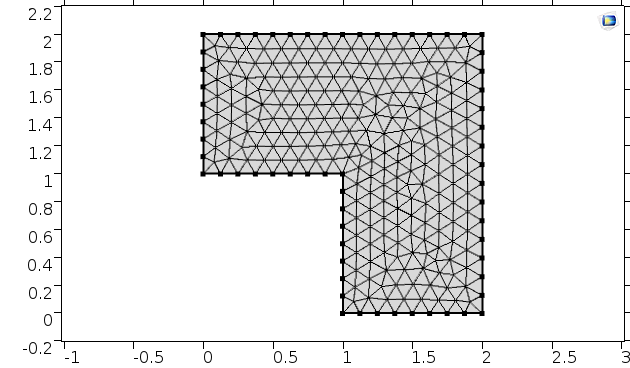
\includegraphics[scale=0.6]{Lmesh.png}
\caption{Geometry and mesh for the L-shaped domain}
\label{Lmesh}
\end{center} 
\end{figure}

This mesh contains 489 triangles. The solution computed by Comsol is given in figure \ref{laplaceL}.

\begin{figure}
\begin{center}
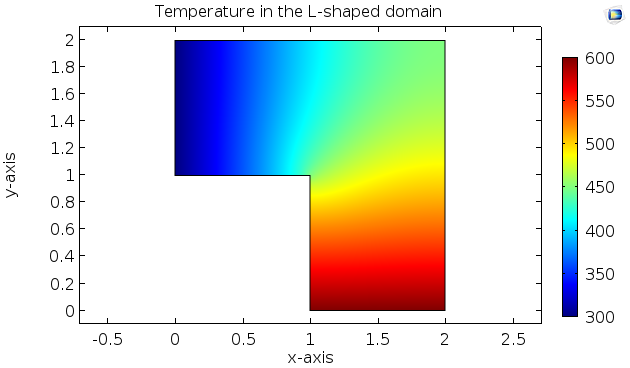
\includegraphics[scale=0.6]{laplaceL.png}
\caption{Solution for the L-shaped domain}
\label{laplaceL}
\end{center}
\end{figure}